\documentclass[a4paper]{article}
\usepackage{preamble}

% Setup title
\title{MATHEMATICS 2 - TERM 2}
\author{Marc Sanchis}
\date{April 2024 - June 2024}

\begin{document}

% Title
\newgeometry{top=2cm, bottom=5.5cm}
\maketitle

% Table of Contents
\renewcommand{\contentsname}{}
\tableofcontents

% Body
\newpage
\restoregeometry
\pagestyle{fancy}
\setcounter{section}{5}

% Counters
\newcounter{ex}[section]
\newcounter{prob}[section]
\setcounter{ex}{0}
\setcounter{prob}{0}

\section{Introduction to Differential Equations}
\setcounter{equation}{0}

A differential equation (DE) is an equation containing one or more dependent variable derivatives, like \textit{Newton's Law}
$$
F=m \frac{d^{2}x(t)}{dt^{2}}=mx''=m\ddot{x}
$$

DEs with one independent variable are called \textbf{Ordinary Differential Equations} (ODE); an example can be the \textit{Radioactive Disintegration} $m'=km$, where $k$ is an independent variable.

DEs with multiple independent variables and partial derivatives are called \textbf{Partial Differential Equations}; an example can be the \textit{Wave Equation}
$$
\nabla u\equiv\nabla^{2}u=\frac{\partial^{2}u(\mathbf{x}, t)}{\partial x^{2}}+\frac{\partial^{2}u(\mathbf{x},t)}{\partial y^{2}}+\frac{\partial^{2}u(\mathbf{x},t)}{\partial z^{2}}=\frac{1}{c^{2}}\frac{\partial^{2}u(\mathbf{x},t)}{\partial t^{2}}
$$

\vspace{1ex}\note{The largest order of derivative defines the order of the DE. An ODE is lineal for $F(t,y,y',\dots,y(n))=0$}\vspace{1ex}

An ODE can be solved with a general ($=\dots+C$) or particular ($=\dots+k,\,k=\mathbb{R}$). The result can be given by an Initial Value Problem (IVP): a function $f(t)$ verifying the ODE and the Initial Condition (IC).

\vspace{1ex}\note{Frontier problems are an IVP but verifying an IC relative to the contour, a Contour Condition (CC)}\vspace{1ex}

\section{First Order Differential Equations}
\setcounter{equation}{0}

\subsection{Separable DE}
\setcounter{equation}{0}

A first-order ODE $F(t,y,y')$ is \textit{separable} if it can be written as
$$
A(t)dt=B(y)dy,\hspace{4ex}y'=\frac{A(t)}{B(y)},\hspace{4ex}y'=C(t)D(y)
$$

\stepcounter{prob}\vspace{2ex}\textit{\textbf{Prob.\thesection.\theprob:}} A bowl filled with water spins at a $w$ velocity. If we put a mass $m$ on the surface of the water and denote tension force by $T$, centrifugal force by $F_{c}$ and weight by $P$. Formulate Newton's Equation.

\begin{align}
F&=ma, & v&=cte\implies a=0 \\
F&=0, & \sum^{}_{}F&=P+F_{c}+T \\
0&= P+F_{c}+T
\end{align}
$$
P=-mg\mathbf{j},\, F_{c}=mR\omega 2i,\, T=-T\sin \alpha \mathbf{i} + T\cos \alpha \mathbf{j}
$$
Where $T=\mid\mid \mathbf{T}\mid\mid$ and $\alpha$ is the angle between the tangent and the horizontal axis

\begin{minipage}{0.4\textwidth}
equalling these terms
\begin{align}
\begin{cases}
T\sin \alpha=mR\omega^{2}, \\
T\cos \alpha=mg
\end{cases} \\
R\omega^{2}g=\tan \alpha
\end{align}
$$
\boxed{\frac{\omega^{2}}{g}x=\frac{dy}{dx}}
$$
\end{minipage} \hfill \begin{minipage}{0.4\linewidth}
\begin{figure}[H]
    \centering
    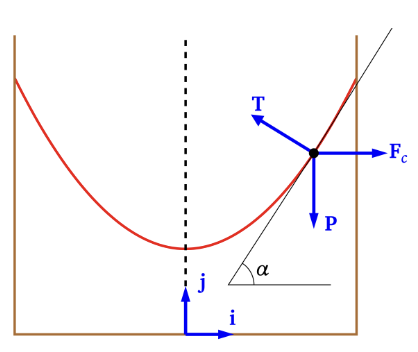
\includegraphics[width=\textwidth]{IMG/ex_water.png}
    \caption{Water bowl example}
    \label{fig:ex_water}
\end{figure}
\end{minipage}



\subsection{Homogeneous ODE}
\setcounter{equation}{0}

\vspace{1ex}\note{A function $f(x,y)$ is said to be of order $n$ if $f(\lambda x,\lambda y)=\lambda^nf(x,y)$}\vspace{1ex}

A first-order ODE $M(x,y)dx+N(x,y)dy=0$ is homogeneous if and only if $M$ and $N$ are of the same order.

\vspace{1ex}\note{Given a homogeneous ODE $dy / dt=f(t,y)$, it can be solved by making the change $u=y / t$ converting the equation into a separable variables equation}\vspace{1ex}

\stepcounter{ex}\vspace{2ex}\textit{\textbf{Ex.\thesection.\theex:}} $t^{3}y'=t^{2}y-2y^{3}$
\begin{align} 
y'=\frac{t^{2}y-2y^{3}}{t^{3}}&=\frac{y}{t}-2\left( \frac{y}{t} \right)^{3} \\
u&=y / t \\
f(y / t)&=f(u)=u-2u^{3} \\
y'=\frac{dy}{dt}&=\frac{d(ut)}{dt}=\frac{du}{dt}t+u \\
\frac{du}{dt}t+u&=u-2u^{3} \\
\frac{du}{2u^{3}}&=-\frac{dt}{t}
\end{align}

\stepcounter{prob}\vspace{2ex}\textit{\textbf{Prob.\thesection.\theprob:}} Find the form of a curved mirror that divides a beam of light parallel to the $X$ axis.

The beams will be reflected towards a point we will be calling $F$ (property of a parabolic antenna).

\begin{figure}[H]
    \centering
    \begin{subfigure}{0.3\textwidth}
        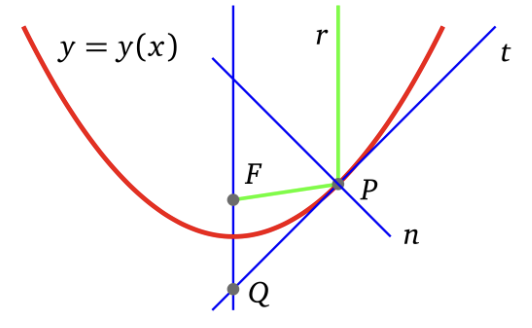
\includegraphics[width=\textwidth]{IMG/prob_mirror1.png}
    \end{subfigure}\hspace{5ex}
    \begin{subfigure}{0.3\textwidth}
        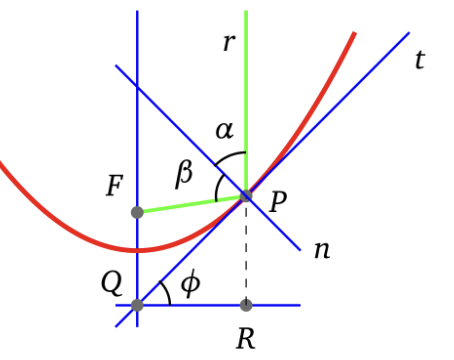
\includegraphics[width=\textwidth]{IMG/prob_mirror2.png}
    \end{subfigure}
    \caption{Parabolic mirror problem}
    \label{fig:prob_mirror}
\end{figure}

Let the axis through $\overline{FQ}$ be $y$, $P(x,y)$ is the intersection of the beam and the mirror, $t$ being its tangent and $n=\mid\mid t\times y(x)\mid\mid$ the normal. The angles denoted by $\alpha,\beta,\phi$. For $r \perp x \implies \phi=\alpha$, and following \textit{Snell's Law} $\alpha=\beta$, and by geometry $\alpha=\phi$, so $\alpha=\beta=\phi$. Knowing this, we can affirm that the triangle formed by $PQF$ is isosceles, implying $PF=FQ$.

$\phi=dy / dx=\frac{PR}{QR}$ and if we place $F$ on $(0,0)$, then $PR=y+FQ=y+\sqrt{ x^{2}+y^{2} }$ and $QR=x$, so
$$
\frac{dy}{dx}=\frac{y+\sqrt{ x^{2}+y^{2} }}{x}\hspace{4ex}\leftarrow\text{homogeneous}
$$
and we can make $u=y / x$
\begin{align}
\frac{d(ux)}{dx}&=\frac{ux+\sqrt{ x^{2}+(ux)^{2} }}{x}\implies \\
\implies&u+x \frac{du}{dx}=u+\sqrt{ 1+u^{2} }\implies \\
\implies&x \frac{du}{dx}=\sqrt{ 1+u^{2} } \implies
\end{align}
$$
\boxed{\frac{du}{\sqrt{ 1+u^{2} }}=\frac{dx}{x} \implies F(y / x)=\log x+C}
$$

\stepcounter{ex}\vspace{2ex}\textit{\textbf{Ex.\thesection.\theex:}} Solve for $y'=(2y-t+1) / (t+y+3)$
\begin{align}
f(\lambda y,\lambda t)&=\frac{2\lambda y-\lambda t+1}{\lambda y+\lambda t+3}, & &\leftarrow\text{not homogeneous}
\end{align}
$$
y=Y+a,\hspace{4ex}t=T+b,\hspace{4ex}a,b=\mathbb{R}
$$
\begin{align}
\frac{dY}{dT}&=\frac{2(Y+a)-(T+b)+1}{(Y+a)+(T+b)+3}= \\
&= \frac{2Y-T+(2a-b+1)}{Y+T+(b+a+3)}
\end{align}

For the equation to be homogeneous, we must solve
$$
\begin{cases}
2a-b+1=0, \\
b+a+3=0
\end{cases}\implies \begin{cases}
a=-4 / 3, \\
b=-5 / 3
\end{cases}
$$
$$
\boxed{\frac{dY}{dT}=\frac{2Y-T}{Y+T}}\hspace{4ex}\leftarrow\text{homogeneous}
$$

\stepcounter{prob}\vspace{2ex}\textit{\textbf{Prob.\thesection.\theex:}} Solve the equation above \textbf{TODO}

\stepcounter{ex}\vspace{2ex}\textit{\textbf{Ex.\thesection.\theex:}} Solve for $y'=(2y-t+1) / (y+t+3)$
\begin{align}
f(\lambda y,\lambda t)&=\frac{2\lambda y-\lambda t+1}{\lambda y+\lambda t+3}\hspace{4ex}\leftarrow\text{not homogeneous} \\
y'=\frac{dy}{dt}&=\left\langle\begin{cases}
2y+6t=1, \\
3y+9t=0
\end{cases}\right\rangle =\frac{2(y+3t)-1}{3(y+3t)} \hspace{4ex}\leftarrow\text{parallel functions}
\end{align}

As the functions are parallel, the previous method will not work, but we can make a variable change $u=y+3t$
$$
\boxed{\frac{du-3\,dt}{dt}=\frac{2u-1}{3u}}
$$
\stepcounter{prob}\vspace{2ex}\textit{\textbf{Prob.\thesection.\theprob:}} Solve the above equation

\subsection{Exact DEs}
\setcounter{equation}{0}
An $M(t,y)dt+N(t,y)dy=0$ DOE is \textit{exact} if its \textit{potential function} $F(t,y)$ exists as
$$
\frac{\partial F}{\partial t}=M(t,y),\hspace{4ex} \frac{\partial F}{\partial y}=N(t,y)
$$
for an \textit{exact DOE} 
$$
F(t,y)=\text{const}
$$

To prove this on any equation of this style
$$
\frac{\partial M}{\partial y}=\frac{\partial N}{\partial t}
$$
\stepcounter{ex}\vspace{2ex}\textbf{\textit{Ex.\thesection.\theex: }}Solve $(2ty+3t^{2}y^{2}+1)dt+(t^{2}+2t^{3}y+2y)dy=0$ 
$\triangleright$ Define $M(y,t)=2ty+3t^{2}y^{2}+1$ and $N(y,t)=t^{2}+2t^{3}+2y$ and observe
$$
\partial_{t}F=2t+6t^{2}y=\partial_{y}N\hspace{4ex}\leftarrow\text{Exact DOE}
$$
$\triangleright$ Find $F(y,t)$
\begin{align}
\text{Exact DOE}\implies \partial _{t}F&=M(y,t)=2ty+3t^{2}y^{2}+1 \\
\partial_{y}F&=N(y,t)=t^{2}+2t^{3}y+2y
\end{align}
$\triangleright$ Integrate
\begin{align}
F(y,t)=\int (2ty+3t^{2}y^{2}+1) \, dt\, =yt^{2}+t^{3}y^{2}+t+g(y)
\end{align}
$\triangleright$ Determine $g(y)$
\begin{align}
\partial_{y}F=t^{2}+2t^{3}y+\frac{dg}{dy}&=N(y,t)=t^{2}+2t^{3}y+2y \\
\frac{dg}{dy}&=2y \\
g(y)&=y^{2}+C \\
\end{align}
$\triangleright$ Solve with $g(y)$
\begin{align}
F(y,t)=yt^{2}+t^{3}y^{2}+t+y^{2}+C=K'
\end{align}
$$
\boxed{K=yt^{2}+t^{3}y^{2}+t+y^{2}}
$$
\stepcounter{prob}\vspace{2ex}\textbf{\textit{Prob.\thesection.\theprob: }}Solve (using $N$) $(3y+2)dt+(8t+8y)dy=0$
$\triangleright$ $M(y,t)$ and $N(y,t)$ already defined, find $F(y,t)$ 
\begin{align}
\text{Exact DOE}\implies \partial_{y}F(y,t)&=N(y,t) \\
F(y,t)&=\int (3t+8y) \, dy\, =3ty+4y^{2}+g(t)
\end{align}
$\triangleright$ Determine $g(t)$
\begin{align}
\partial_{t}F(y,t)=3y+&0+\frac{dg}{dt}=3y+2 \\
g(t)&=2t+C
\end{align}
$\triangleright$ Solve with $g(t)$ 
\begin{align}
F(y,t)=3ty+4y^{2}+2t+C=K'
\end{align}
$$
\boxed{K=3ty+4y^{2}+2t}
$$

\subsection{Integral Factor}
\setcounter{equation}{0}

An integral factor is a $\mu = \mu(t,y)$ function such that 
$$
\mu Mdt+\mu Ndy=0
$$
making the original $Mdt+Ndy=0$ solvable.

These functions are difficult to find and only two will be showed in this class.

\subsubsection{First type}

For $\mu = \mu(t)$
\begin{align}
    \partial_y(\mu M)&=\partial_t(\mu N) \\
    \partial_t(\mu N)&=D_t(\mu) N+\mu \partial_tN \\
    \mu \partial_yM&=D_t(\mu)N+\mu \partial_tN \\
    \mu\left(\partial_yM-\partial_tN\right)&=D_t(\mu)N \\
    \frac{1}{N}\left(\partial_yM-\partial_tN\right)dt&=D_\mu \mu
\end{align}

\stepcounter{ex}\vspace{2ex}\textit{\textbf{Ex.\thesection.\theprob:}} $(t+y)dy-ydt=0$
\begin{align}
    \partial_yM&=-1 \\
    \partial_tN&=1 \\
    \partial_yM&\neq \partial_tN \\
    \frac{1}{N}\left(\partial_yM-\partial_tN\right)dt&=D_\mu\mu \\
    \frac{-2}{t+y}dt&=D_\mu\mu \leftarrow\text{Dependant on }t,y
\end{align}
As the left side is not only dependant on $t$, the $\mu$ function can not exist.

\stepcounter{ex}\vspace{2ex}\textit{\textbf{Ex.\thesection.\theprob:}} $(1-y)dt+(1+t)dy=0,\,y(0)=0$
\begin{align}
    \frac{1}{N}\left(\partial_yM-\partial_tN\right)dt&=D_\mu\mu \\
    \frac{-2}{1+t}dt&=D_\mu\mu \\
    -2\int\frac{1}{1+t}\,dt&=\int\frac{1}{\mu}\,d\mu \\
    \log \mu&=-2\log (1+t) \\
    \mu(t)&=(1+t)^{-2}
\end{align}
now we multiply the original expression with the $\mu$ we found
\begin{align}
    \frac{1-y}{(1+2)^2}dt+\frac{1+t}{(1+t)^2}dy=0
\end{align}
there exists a function $F(t,y)$ such that
\begin{align}
    \partial_tF=\frac{1-y}{(1+t)^2},\hspace{4ex}\partial_y\frac{1}{1+t}
\end{align}
the first function depends on two variables, so the second will be used now
\begin{align}
    F(t,y)&=\int \frac{1}{1+t}dy=\frac{y}{1+t}+g(t)\\ 
    \partial_tF&=\frac{-y}{(1+t)^2}+D_tg=\frac{1-y}{(1+t)^2}\implies g(t)=-\frac{1}{1+t}+C \\
    F(t,y)&=\frac{y}{1+t}-\frac{1}{1+t}+C \\
    K&=\frac{y}{1+t}-\frac{1}{1+t}=0 \\
    0&=\frac{y}{1+t}-\frac{1}{1+t}
\end{align}
$$
\boxed{y=1}
$$

\subsubsection{Second type}

For $\mu=\mu(y)$, doing the inverse path for the \textit{First Type}
\begin{align}
    \frac{1}{M}\left(\partial_tN-\partial_yM\right)dy&=D_\mu\mu
\end{align}

\stepcounter{ex}\vspace{2ex}\textit{\textbf{Ex.\thesection.\theprob:}} $(y+t^2)dy=2ydt$
If we try solving via the \textit{First Type}
\begin{align}
    \frac{1}{N}\left(\partial_yM-\partial_tN\right)dt&=D_\mu\mu \\
    \frac{-4t}{y+t^2}dt&=D_\mu\mu \leftarrow\text{Dependant on }t,y
\end{align}
as the left side is dependant on multiple variables $\mu$ can not exist, but if we use the \textit{Second Type} way
\begin{align}
    \frac{1}{M}\left(\patchcmd_tN-\partial_yM\right)dy&=D_\mu\mu \\
    \frac{-2}{y}dy&=D_\mu\mu 
\end{align}
this way $\mu$ exists
\begin{align}
    \log\mu &= -2\log y \\
    \mu &=y^{-2} \\
    \frac{2t}{y}dt-\frac{y+t^2}{y^2}dy&=0
\end{align}
$$
\boxed{\mu(y)=1/y^2}
$$

\subsection{Lineal Equations}
\setcounter{equation}{0}

A Lineal Equation (LE) is defined by a DE expressible as $y'+p(t)y=q(t)$. To solve a Lineal Ordinal Differential Equation (LODE), it is multiplied by $\mu=e^{ \int p(t) \, dt\, }$  and try to get the derivative of a product with $\mu'$ in function of $\mu$ on the other side, like so
$$
\mu'=D_{t}\mu=e^{ \int p(t) \, dt\,  }p(t)=\mu p
$$
\begin{align}
\mu y'+\mu py=\mu p\implies \mu y'+\mu'y=\mu q\implies(\mu y)'=\mu q
\end{align}
then the expression can be integrated
\begin{align}
\mu y=\int \mu q \, dt\, \implies
\end{align}
$$
\boxed{y=\frac{1}{\mu}\int \mu q \, dt\, }
$$
\vspace{1ex}\note{$\mu$ is a function of $t$ and can not be moved in or out of the integral}\vspace{1ex}

\stepcounter{ex}\vspace{2ex}\textbf{\textit{Ex.\thesection.\theex: }}Solve $y'+2y=e^{t}$

$\triangleright$ Determine linearity and define $p(t)$ and $q(t)$
$$
\text{Linear}\implies p(t)=2,\hspace{4ex}q(t)=e^{ t }
$$
$\triangleright$ Find $\mu=e^{ \int p(t) \, dt\, }$
\begin{align}
\int p(t) \, dt\, =\int 2 \, dt\, =2t\implies \mu=e^{ 2t }
\end{align}
$\triangleright$ $\mu'$ in function of $\mu$
\begin{align}
\mu'=2\mu
\end{align}
$\triangleright$ Multiply by $\mu$ and obtain the derivative on the other side
\begin{align}
\mu y'+\mu 2y=\mu e^{ t }\implies(\mu y)'=\mu e^{ t }
\end{align}
$\triangleright$ Solve by obtaining $y$
\begin{align}
\mu y=\int \mu e^{ t } \, dt\, &=\int e^{ 2t }e^{ t } \, dt\, =\int e^{ 3t } \, dt\, =\frac{e^{ 3t }}{3}+C \\
y&=\frac{1}{e^{ 2t }}\left( \frac{e^{ 3t }}{3}+C \right)
\end{align}
$$
\boxed{y=\frac{e^{ t }}{3}+C\,e^{ -2t }}
$$

\stepcounter{prob}\vspace{2ex}\textbf{\textit{Prob.\thesection.\theprob: }}Solve $(y+x^{2}\cos x)dx-xdy=0$ 
$\triangleright$ Define $M(x,y)=y+x^{2}\cos x$ and $N(x,y)=-x$
$$
D_{y}M(x,y)=1,\hspace{4ex}D_{x}N(x,y)=-1 \hspace{4ex}\leftarrow\text{Not exact DOE}
$$
$\triangleright$ Determine linearity and find $p(x)$ and $q(x)$
\begin{align}
(y+x^{2}\cos x)+xy'&=0 \\
(y+x^{2}\cos x)&=xy' \\
\left( \frac{y}{x}+x\cos x \right)&=y' \\
y'-\frac{y}{x}=x\cos x
\end{align}
$$
p(x)=-\frac{1}{x},\hspace{4ex}q(x)=x\cos x
$$
$\triangleright$ Find $\mu$
\begin{align}
\int p(x) \, dx\, &=\int -\frac{1}{x} \, dx\, =-\log x \\
\mu&=e^{ -\log x }=\frac{1}{x}
\end{align}
$\triangleright$ Express $\mu'$ in function of $\mu$
\begin{align}
\mu'=-\frac{\mu}{x}
\end{align}
$\triangleright$ Multiply by $\mu$ and find the derivative on the other side
\begin{align}
\mu y'+\frac{\mu y}{x}=\mu x\cos x \implies (\mu y)'=\cos x
\end{align}
$\triangleright$ Solve by obtaining $y$
\begin{align}
\mu y&=\int \cos x \, dx\, =\sin x+C  \\
y(x)&=\mu^{-1}\sin x+C
\end{align}
$$
\boxed{y(x)=x(\sin x+C)}
$$

\subsection{Curve Family}
\setcounter{equation}{0}

An expression $F(x,y,K)=0,\,K\in\mathbb{Z}$ defines a Curve Family.

\subsubsection{Orthogonal Trajectory}
A curve from a Curve Family with an orthogonal intersection with each of the other curves.

\begin{figure}[H]
    \centering
    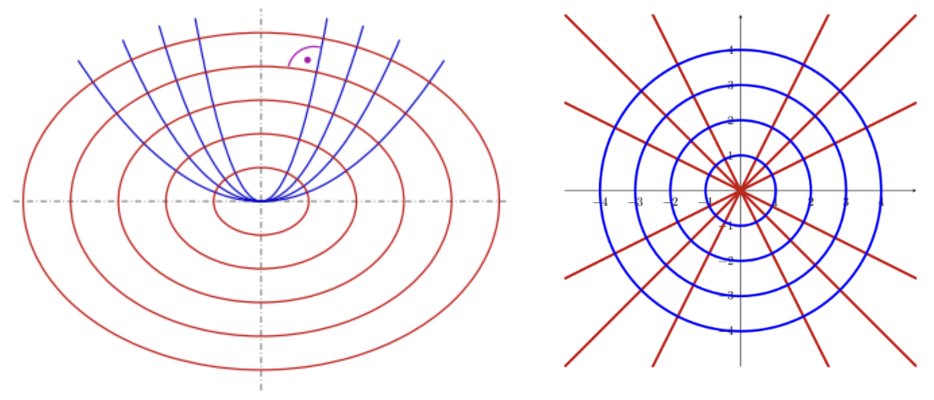
\includegraphics[width=0.5\textwidth]{IMG/ortho_fam.png}
    \caption{Curves of an Orthogonal Family}
    \label{fig:ortho_fam}
\end{figure}

\stepcounter{ex}\vspace{2ex}\textbf{\textit{Ex.\thesection.\theex: }}Circumference contour
$$
x^{2}+y^{2}=R^{2}
$$
\begin{align}
x^{2}+y^{2}+R^{2}&=0 \\
F(x,y,K)&=0 \\
D_{x}F(x,y,K)&=2x+2yy'
\end{align}
$$
\boxed{x+yy'=0}
$$
\vspace{1ex}\note{The orthogonal family follows $y'=\frac{y}{x}$}\vspace{1ex}

\begin{align}
y'=\frac{y}{x}&=\int \frac{1}{y} \, dy\, =\int \frac{1}{x} \, dx\,  \\
\ln y&=\ln x+C \\
e^{ \ln y }&=e^{ \ln x+C }
\end{align}
$$
\boxed{y=xe^{ C }}\hspace{4ex}\leftarrow\text{y=Kx}
$$

\subsubsection{Orthogonal Trajectories With Polar Coordinates}
Polar coordinates describe curves differently to Cartesian coordinates
\begin{table}[H]
    \centering
    \begin{tabular}{c|c|c}
        & Cartesian & Polar \\ \hline
        Origin-centred circumferences & $x^2+y^2=C^2$ & $\rho=C$ \\ \hline
        Semi-line through the origin & $y=kx$ & $\theta=C$ \\ \hline
        Lines parallel to the $X$ axis & $y=k$ & $\rho\sin\theta=k$
    \end{tabular}
    \caption{Cartesian vs. Polar}
    \label{tab:polars}
\end{table}

\section{Superior Order ODEs}
\setcounter{equation}{0}
\subsection{Constant coefficient ODEs}
\setcounter{equation}{0}
$a_{n}(t)D_{t}^{n}y+a_{n-1}D_{t}^{n-1}y+\dots+a_{1}D_{t}y=b(t)$ is the form of an ODE of order $>1$, it always has a solution for $b(t)=0$: $a_{n}(t)D_{t}^{n}y+a_{n-1}D_{t}^{n-1}y+\dots+a_{1}D_{t}y=\boxed{0}$ .

In order to solve one, the solution of the homogeneous and one of the particulars
$$
\sum^{n}_{k=0}a_{k}(y_{h}+y_{p})=0+b(t)=b(t)
$$
\vspace{1ex}\note{Note that the sum of only one of the homogeneous solutions with the homogeneous will be the general solution}\vspace{1ex}

\stepcounter{ex}\vspace{2ex}\textbf{\textit{Ex.\thesection.\theex: }}$a_{1}y'+a_{0}y=0$
\begin{align}
\frac{y'}{y}&=- \frac{a_{0}}{a_{1}} \\
\int \frac{y'}{y} \, dt\, &=-\int \frac{a_{0}}{a_{1}} \, dt\,  \\
\ln y &= -\frac{a_{0}}{a_{1}}t+C \\
y(t)&=Ke^{ -\frac{a_{0}}{a_{1}}t }
\end{align}

And using $\mu$
\begin{align}
y'+p(t)&=q(t) \leftarrow\text{Desired form} \\
\implies a_{1}y'+a_{0}y=0 &\implies y'+\frac{a_{0}}{a_{1}}y=0 \\
\mu=e^{ \int p(t) \, dt\,  }&=e^{ \frac{a_{0}}{a_{1}}t } \\
\end{align}
now applying $\mu y'+\mu \frac{a_{0}}{a_{1}}y=0$
\begin{align}
e^{ \frac{a_{0}}{a_{1}}t }y'+e^{ \frac{a_{0}}{a_{1}}t } \frac{a_{0}}{a_{1}}y &= D_{t}\left( e^{ \frac{a_{0}}{a_{1}} }y \right)=0 \\
y(t)&=Ke^{ - \frac{a_{0}}{a_{1}}t }
\end{align}
$$
\boxed{y(t)=Ke^{ -\frac{a_{0}}{a_{1}}t }}
$$
To find the characteristic polynomial
$$
a_{n}\lambda^{n}+a_{n-1}\lambda^{n-1}+\dots a_{0}=0\implies \lambda_{1},\lambda_{2},\lambda_{3},\dots
$$

\stepcounter{ex}\vspace{2ex}\textbf{\textit{Ex.\thesection.\theex: }}

$\triangleright\, 3y'''-2y'=0$
\begin{align}
3\lambda^{3}e^{ \lambda t }-2\lambda e^{ \lambda t }&=0 \\
3\lambda^{3}-2\lambda&=0 \\
\end{align}
$$
\boxed{3\lambda^{3}-2\lambda=0}
$$

$\triangleright\,y''-3y'+2y=0$
\begin{align} 
\lambda^{2}-3\lambda+2&=0 \\
\lambda=\frac{3\pm \sqrt{ 9-8 }}{2} &=\frac{3\pm1}{2}\begin{cases}
\lambda_{1}=2 \\
\lambda_{2}=1
\end{cases} \\
y_{h}(t)=C_{1}y_{1}+C_{2}y_{2}&=C_{1}e^{ 2t }+C_{2}e^{ t }
\end{align}
$$
\boxed{y_{h}(t)=C_{1}e^{ 2t }+C_{2}e^{ t }}
$$

\stepcounter{prob}\vspace{2ex}\textbf{\textit{Prob.\thesection.\theprob: }}

$\triangleright\, y''+y'=0,\,y(0)=1,\,y'(0)=0$

The ODE is homogeneous and has constant coefficients $\to e^{ \lambda t }$
\begin{align}
\lambda^{2}+\lambda&=0 \\
\lambda(\lambda+1)&=0\begin{cases}
\lambda_{1}=0 \\
\lambda_{2}=-1
\end{cases} \\
\begin{cases}
y_{1}(t)&=e^{ 0t }=1 \\
y_{2}(t)&=e^{ -t } 
\end{cases}&\implies \begin{cases}
y_{1}(0)=C_{1}+C_{2}=1 \\
y'(0)=-C_{2}=0
\end{cases}
\end{align}
$\triangleright\, y'''-5y''+6y'=0$

Homogeneous with constant coefficients $\to e^{ \lambda t }$
\begin{align}
\lambda^{3}-5\lambda^{2}+6\lambda&=0 \\
\lambda(\lambda^{2}-5\lambda+6)&=0 \\
\lambda=\frac{5\pm \sqrt{ 25-24 }}{2}&=\frac{5\pm1}{2}\begin{cases}
\lambda=3 \\
\lambda=2
\end{cases} \\
y_{h}(t)=C_{1}&+C_{2}e^{ 3t }+C_{3}e^{ 2t }
\end{align}
$$
\boxed{y_{h}(t)=C_{1}+C_{2}e^{ 3t }+C_{3}e^{ 2t }}
$$

$\triangleright\, y'''+3y''=4y$

\begin{align}
y'''+3y''-4y&=0 \\
\lambda^{3}+3\lambda^{2}-4&=0 \\
\text{Rufini}\to &\begin{cases}
\lambda=1 & \text{Simple} \\
\lambda=-2 & \text{Double}
\end{cases} \\
y(t)=C_{1}e^{ t }+&C_{2}e^{ -2t }+C_{3}te^{ -2t }
\end{align}
$$
\boxed{y(t)=C_{1}e^{ t }+C_{2}e^{ -2t }+C_{3}te^{ -2t }}
$$
\subsubsection{Complex arrays}
\setcounter{equation}{0}

\stepcounter{ex}\vspace{2ex}\textbf{\textit{Ex.\thesection.\theex: }}$y''+2y'+2y=0$

\begin{align}
\lambda^{2}+2\lambda+2&=0 \\
\lambda=\frac{-2\pm \sqrt{ -4 }}{2}&=-1\pm i \begin{cases}
\lambda=-1+i \\
\lambda=-1-i
\end{cases}
\end{align}
$$
y_{1}(t)=e^{ (-1+i)t }
$$
In this case \textit{Euler's Formula} can be applied
$$
\text{Euler's Formula }\to e^{\alpha t}=\cos(\alpha)+i\sin(\alpha) 
$$
\begin{align}
\text{Euler's Formula }\to y_{1} (t)&=e^{ -t }(\cos t+i\sin t)= \\
&=\overbrace{e^{ -t }\cos t}^{\text{Real}}+\overbrace{i\,e^{ -t}\sin t}^{\text{Im}}
\end{align}
\begin{align}
y_{1}(t)&=C_{1}e^{ (-1+i)t }+C_{2}e^{ (-1-i )t}= \\
&=C_{1}e^{ -t }\cos t+iC_{1}e^{ -t }\sin t+C_{2}e^{ -t }\cos t-iC_{2}e^{ -t }\sin t= \\
&=(C_{1}+C_{2})e^{ -t }\cos t+i(C_{1}-C_{2})e^{ -t }\sin t
\end{align}

\textbf{\textit{Ex. Page 17}}

\setcounter{equation}{0}
\stepcounter{prob}\vspace{2ex}\textbf{\textit{Prob.\thesection.\theprob: }}$y''+ay=0,\,y(1)=y(0)=0$
\begin{align}
&\lambda^{2}+a=0 \\
&\lambda=\pm \sqrt{ -a }\begin{cases}
a=0,&\lambda=0\,\leftarrow\text{(Double)} \\
a>0,&\lambda=\pm\sqrt{ |a| } \\
a<0,&\lambda=\pm\sqrt{ |a| }
\end{cases} \\
&\begin{cases}
\lambda=0\implies e^{ 0t },\,te^{ 0t } & \begin{cases}
y(0)=C_{1}=0 \to \boxed{\text{null}}\\
y(1)=C_{1}+C_{2}t=0+C_{2}=0 \to \boxed{\text{null}}
\end{cases} \\
\lambda=\sqrt{ |a| }\implies C_{1}e^{ -\sqrt{ |a| } }+C_{2}e^{ +\sqrt{ |a| } } & \begin{cases}
y(0)=C_{1}+C_{2}=0 \to \boxed{\text{null}}\\
y(1)=C_{1}e^{ -\sqrt{ |a| } }+C_{2}e^{ +\sqrt{ |a| } } \implies\dots
\end{cases}
\end{cases}
\end{align}
\begin{align}
\dots y(1)&=0=C_{1}\cos \sqrt{ |a| }+C_{2}\sin \sqrt{ |a| }=C_{2}\sin\left(\sqrt{ |a| }\right)=0 \\
\sqrt{ |a| }&=n\pi \iff y(t)=C_{2}\sin\left( n\pi t\right)
\end{align}
$$
\boxed{\sqrt{ |a| }=n\pi,\,y(t)=C_{2}\sin(n\pi t)}
$$

\stepcounter{prob}\vspace{2ex}\textbf{\textit{Prob.\thesection.\theprob: }}$y^{(4)}+2y''+y=0$
\begin{align}
\lambda^{4}+2\lambda^{2}+1&=0 \\
\langle \mu=\lambda^{2} \rangle \to \mu^{2}+2\mu+1&=0 \\
\mu=\frac{-2\pm \sqrt{ 4-4 }}{2}&=-1\leftarrow\text{(Double)} \\
\langle \mu=-1\text{ (Double)} \rangle \to \lambda=\pm \sqrt{ -1 }&=\pm i\begin{cases}
\lambda=+i\text{ (Double)},&e^{ it },te^{ it } \implies\dots\\
\lambda=-i\text{ (Double)},&e^{ -it },te^{ -it }
\end{cases} \\
\dots \begin{cases}
e^{ it }=\cos t+i\sin t \\
te^{ it }=t\cos t+it\sin t
\end{cases}\implies y(t)&=C_{1}\cos t+C_{2}\sin t+C_{3}\cos t+C_{4}\sin t
\end{align}
$$
\boxed{y(t)=C_{1}\cos t+C_{2}\sin t+C_{3}\cos t+C_{4}\sin t}
$$

\stepcounter{prob}\vspace{2ex}\textbf{\textit{Prob.\thesection.\theprob: }}$y'''-y''+y'-y=0$ 
\begin{align}
\lambda^{3}-\lambda^{2}+\lambda-1&=0 \\
\text{Rufini}\to \lambda=\pm1&=(\lambda-1)(\lambda^{2}+1)
\begin{cases}
\lambda=1,&e^{ t }  \\
\lambda=i,&e^{ it } \implies \dots \\
\lambda=-i,&e^{ -it }
\end{cases} \\
\dots e^{ it }=\cos t + i\sin t&\implies y(t)=C_{1}e^{ t }+C_{2}\cos t+C_{3}\sin t
\end{align}
$$
\boxed{y(t)=C_{1}e^{ t }+C_{2}\cos t+C_{3}\sin t}
$$
\subsection{Non-homogeneous ODEs With Constant Coefficients}
\setcounter{equation}{0}

Now, for a non-homogeneous ODE, only one particular solution is needed so it can be added to the homogeneous solution to get the general solution.

\subsubsection{Undetermined Coefficients Method}
\setcounter{equation}{0}
Given a non-homogeneous ODE like
$$
a_{n}y^{(n)}+a_{n-1}y^{(n-1)}+\dots+a_{0}y=b(t)
$$
first, we classify $b(t)$

$\triangleright$ \textbf{\textit{First case:}} If the arrays include $0$ as a $k$ order solution, then the particular solution is
$$
y_{p}=t^{k}(A_{0}+A_{1}t+\dots+A_{m}t^{m})
$$

\stepcounter{ex}\vspace{2ex}\textbf{\textit{Ex.\thesection.\theex: }}$y''+y=t,\,y(0)=1,\,y'(0)=2$
$$
y(t)=y_{p}(t)+y_{h}(t)
$$
\begin{align}
y''+y&=0 \\
\lambda^{2}+1&=0 \\
\lambda&=\pm i\implies e^{ it },e^{ -it } \\
y_{h}(t)&=C_{1}\cos t+C_{2}\sin t \\
\end{align}
$$
b(t)=t,\hspace{4ex}m=1,\hspace{4ex}k=0
$$
\begin{align}
\begin{cases}
y_{p}(t)&=t^{0}(A_{0}+A_{1}t)=A_{0}+A_{1}t \\
y_{p}'(t)&=A_{1} \\
y_{p}''(t)&=0
\end{cases}\implies 0+A_{0}+A_{1}t&=t \\
y_{p}(t)&=t
\end{align}
\begin{align}
y(t)&=C\cos t+i\sin t+t \\
y(0)&=1 & C_{1}=1\\
y'(0)&=2 & y'(0)=2=C_{2}+1\implies C_{2}=1\\
y'(t)&=-C_{1}\sin t+C_{2}\cos t+1
\end{align}

\stepcounter{prob}\vspace{2ex}\textbf{\textit{Prob.\thesection.\theprob: }}$y''+y'=t^{2}+1$

$$
y(t)=y_{p}(t)+y_{h}(t)
$$
\begin{align}
\lambda^{2}+\lambda&=0 \\
\lambda+1&=0\begin{cases}
\lambda=0,&e^{ 0t } \\
\lambda=-1,&e^{ -t }
\end{cases} \\
y_{h}(t)&=C_{1}e^{ 0t }+C_{2}e^{ -t } \\
y_{h}&=C_{1}+C_{2}e^{ -t }
\end{align}
$$
b(t)=t^{2}+1,\hspace{4ex}m=2,\hspace{4ex}k=1
$$
\begin{align}
&\begin{cases}
y_{p}(t)=t^{2}(A_{0}+A_{1}t+A_{2}t^{2}) \\
y_{p}'(t)=(A_{0}+A_{1}t+A_{2}t^{2})+t(A_{1}+2A_{2}t)\\
y_{p}''(t)=A_{1}+2A_{2}t+A_{1}+4A_{2}t
\end{cases}\implies y'+y''=b(t)\dots \\
\dots& \overbrace{A_{0}+2A_{1}t+3A_{2}t^{2}}^{y'}+\overbrace{2A_{1}+6A_{2}t}^{y''}=\overbrace{t^{2}+1}^{b(t)} \\
&3A_{2}t^{2}+(2A_{1}+6A_{2})t+4A_{1}+A_{0}=t^{2}+1
\end{align}
\begin{align}
\begin{cases}
3A_{2}=1&A_{2}=\frac{1}{3} \\
2A_{1}+6A_{2}=0 & A_{1}=-1 \\
2A_{1}+A_{0}=1 & A_{0}=1-2A_{1}=3
\end{cases}
\end{align}
$$
\boxed{y_{p}(t)=3t^{2}-t^{3}+\frac{t^{4}}{3}}
$$

$\triangleright$ \textbf{\textit{Second case:}} For the solution $\neq 0$,
$$
y_{p}(t)=At^{k}e^{ \alpha t }
$$

\stepcounter{ex}\vspace{2ex}\textbf{\textit{Ex.\thesection.\theex: }}$y''+y=e^{ 2t }$
\begin{align}
y_{h}(t)&=C_{1}\cos t+C_{2}\sin t
\end{align}
$$
b(t)=e^{ 2t },\hspace{4ex}k=1,\hspace{4ex}\alpha=2
$$
\begin{align}
\lambda^{2}+1&=0\implies \lambda=\pm i
\end{align}

\end{document}